\chapter{Maven}
\label{chap:maven}

\fcolorbox{black}[HTML]{E9F0E9}{\parbox{\textwidth}{%
\noindent \textbf{Learning goals}\\
The junior-colleague
\begin{enumerate}[nolistsep]
\item can explain what Maven is.
\item can describe the 3 build lifecycles of Maven.
\item can explain that each build lifecycle is made up of phases.
\item can explain that each build phase is made up of plugin goals.
\item can identify the project coordinates.
\item can describe the Maven Standard Directory Layout.
\item can explain what a dependency is.
\item can describe the different dependency scopes.
\item can explain what a transitive dependency is.
\item can explain what a dependency tree is.
\item can execute Maven commands from CLI.
\item can manage dependencies with Maven.
\item understand the role of Maven in a Continuous Integration (CI) pipeline.
\item can configure Maven for automated builds and testing in a CI/CD workflow.
\item can implement a basic CI pipeline using GitHub Actions and Maven.
\end{enumerate}}}

\section{What is Maven?}

Maven is a tool that can be used for building and managing Java-based projects.
Every Java project requires certain dependencies, which are automatically downloaded when using Maven.

The main objectives of using Maven for developers are:
\begin{itemize}
\item Making the build process easy
\item Providing a uniform build system
\item Providing information about project quality (for example unit test reports)
\item Encouraging better development practices
\end{itemize}

Maven is much more than a build tool.  Maven offers support for automatic source generation,  compiling the source code and test sources, packaging final product(s) for different environments, running health checks and reporting.  Continuous builds, integration, and testing can be easily handled by using Maven. A tool commonly used for creating CI/CD pipelines (continuous integration and continuous delivery) is Jenkins.  Jenkins cannot replace Maven or vice-versa. Jenkins can use Maven as its build tool.  
When Jenkins deploys artifacts to remote repositories, they are usually Maven repositories. 

According to Jetbrain's 2023 Java ecosystem report \footnote{\url{https://www.jetbrains.com/lp/devecosystem-2023/java/}} Maven is most popular build tool for the Java ecosystem.

\section{Installation and Configuration}

IntelliJ IDEA has in-built support for Maven.  However we want to make Maven available in the command-line interface. Therefore we need to install Maven. 

 \fcolorbox{black}[HTML]{ADD8E6}{\parbox{\textwidth}{%
\noindent \textbf{Maven download and documentation pages:}\\
Download page: \url{https://maven.apache.org/download.cgi}\\
Installation instructions: \url{https://maven.apache.org/install.html}
}}

Confirm that Maven is installed correctly by executing \fbox{\strut \$mvn -v} in a terminal window. 

\begin{lstlisting}[language=bash, frame=single]
$ mvn -v
Apache Maven 3.8.2 (ea98e05a04480131370aa0c110b8c54cf726c06f)
Maven home: /usr/local/Cellar/maven/3.8.2/libexec
Java version: 17.0.1, vendor: Oracle Corporation, runtime: /Library/Java/JavaVirtualMachines/jdk-17.0.1.jdk/Contents/Home
Default locale: nl_BE, platform encoding: UTF-8
OS name: "mac os x", version: "11.5.2", arch: "x86_64", family: "mac"
\end{lstlisting}


\section{Maven Standard Directory Layout}

When you create a new Maven project, a directory which name matches the artifactId is generated. This directory is known as the project’s base directory. 
Every Maven project has a file named \textbf{pom.xml} which is known as the \textbf{Project Object Model} (POM). This file describes the project, configures plugins, and declares dependencies.
The project’s source code and resources are placed in the folder \textbf{src/main}.
The project’s unit tests are located in \textbf{src/test}.
The target folder is the Maven default output folder. You can delete all the target's folder content with the \fbox{\strut \$mvn clean} command.


\section{Maven architecture}

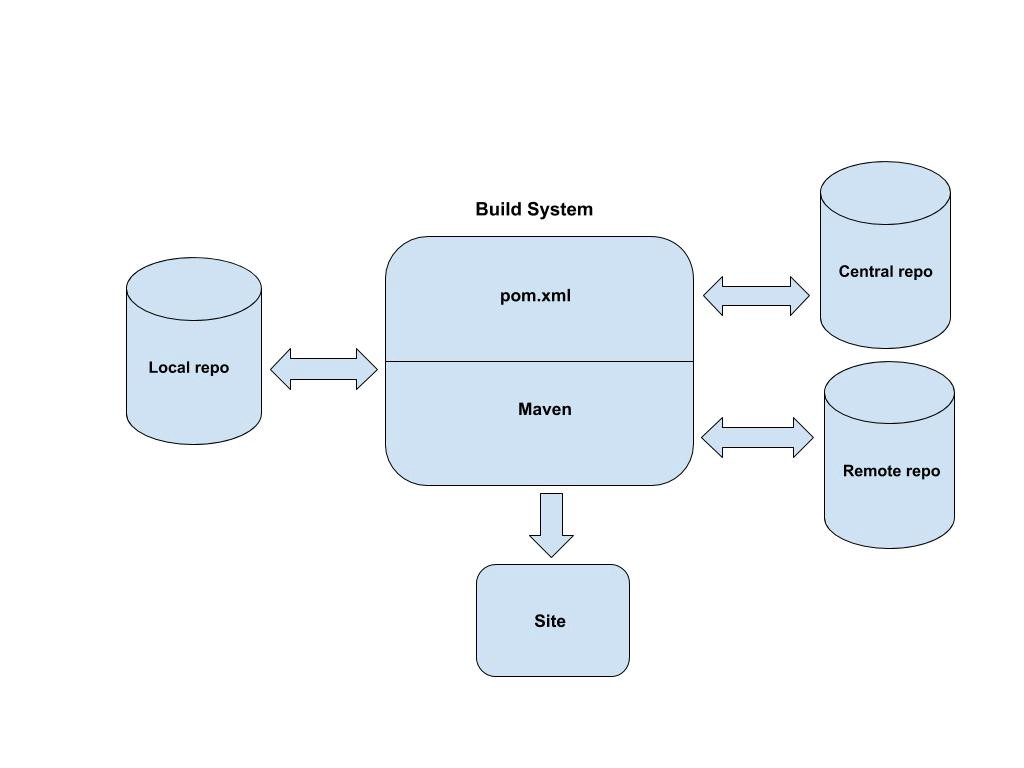
\includegraphics[width=\textwidth]{./images/maven/maven-architecture} 

Central repository is provided by the Maven community. This Central repository contains a large number of common libraries.  Whenever you specify a dependency in pom.xml,  Maven will look for it in the local repository first. If the necessary dependency  isn't included in the local repository, Maven will download it from the Central repository and copy it to your local repository.  Remote repository is a place where developers (or Jenkins) can copy the final packages, so other developer can use these final packages as a dependency in their projects.

Acces to internet is recommended when using Maven, however it is possible to work offline if all dependencies are available in your local repository.


\section{Maven built-in life cycles}

There are three built-in life cycles defined in Maven.  The \textit{default} build life cycle is the main build life cycle.

\begin{tabularx}{\textwidth}{ |l|X|l| } 
\hline
clean & handles the cleanup of directories and files generated during the build process & mvn clean \\ 
default & handles the build and distribution of the project & mvn [plugin:goal]* [phase]* \\ 
site & create project documentation & mvn site \\ 
\hline
\end{tabularx}

To run a specific goal, without executing the entire phase (and the preceding phases) the command \fbox{\strut \$mvn [plugin:goal]} can be used.  Phases on the other hand are executed in a specific order and all the preceding phases are executed as well!

\section{A Build Lifecycle is Made Up Of Phases}

Each life cycle consists of a sequence of phases. The default build lifecycle consists of 23 phases. In the image below the 8 main phases are included. On the other hand, clean lifecycle consists of 3 phases, while the site lifecycle is made up of 4 phases.

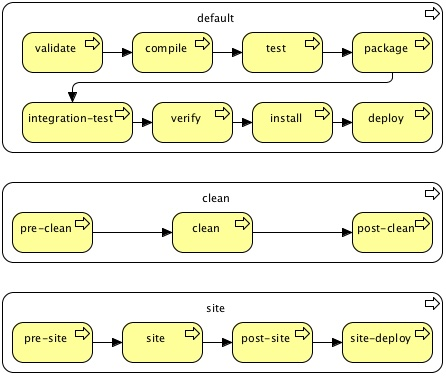
\includegraphics[width=\textwidth]{./images/maven/maven-lifecycles} 

Each phase is responsible for a specific task. Here are the 8 most important phases in the default build lifecycle.

\begin{tabularx}{\textwidth}{ |l|X| } 
 \hline
validate & check if all information necessary for the build is available \\
compile & compile the source code \\
test & run unit tests \\
package & package compiled source code into the distributable format, (jar, war, …)\\
integration-test & process and deploy the package if needed to run integration tests \\
verify & run any checks on results of integration tests to ensure quality criteria are met\\
install & install the package to a local repository\\
deploy & copy the package to the remote repository\\
 \hline
\end{tabularx}

\section{Plugins and Goals}

Maven is actually a plugin execution framework. Every task executed by Maven is actually done by a \textbf{goal}, where goals are grouped together in \textbf{plugins}.  When we run a phase, all the goals bound to the phase are executed in order.

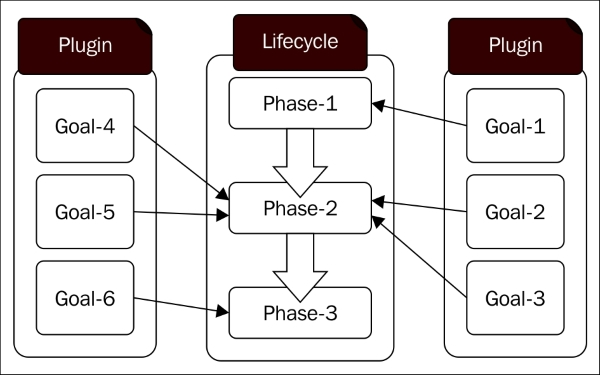
\includegraphics[width=\textwidth]{./images/maven/maven_goals} 

Several phases of the default built-in lifecycles have goals bounded to them.  Due to this default configuration you're able to build a Java project without extra configuration.

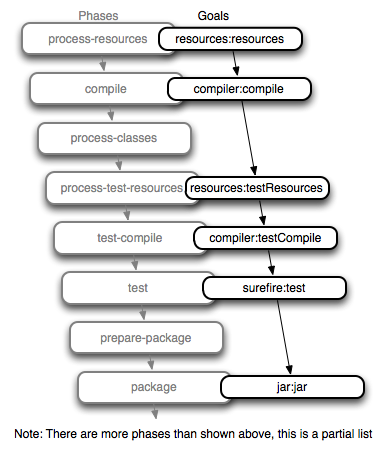
\includegraphics[width=\textwidth]{./images/maven/maven-lifecycle-binding} 

The compile goal from the compiler plugin is bound to the compile phase and is responsible for compiling the source code. The test goal from the surefire plugin is bound to the test phase and is reponsible for running the unit tests.

You can generate an overview of all the phases and the specific goals bounded to these phases by running the command \fbox{\strut \$mvn help:describe -Dcmd=PHASENAME}

\begin{lstlisting}[language=bash, frame=single]
$ cd superhero-backend/
$ mvn help:describe -Dcmd=compile
[INFO] Scanning for projects...
[INFO] 
[INFO] ----------------------< be.pxl:superhero-backend >----------------------
[INFO] Building superhero-backend 0.0.1-SNAPSHOT
[INFO] --------------------------------[ jar ]---------------------------------
[INFO]
[INFO] --- maven-help-plugin:3.3.0:describe (default-cli) @ superhero-backend ---
[INFO] 'compile' is a phase corresponding to this plugin:
org.apache.maven.plugins:maven-compiler-plugin:3.1:compile

It is a part of the lifecycle for the POM packaging 'jar'. This lifecycle includes the following phases:
* validate: Not defined
* initialize: Not defined
* generate-sources: Not defined
* process-sources: Not defined
* generate-resources: Not defined
* process-resources: org.apache.maven.plugins:maven-resources-plugin:2.6:resources
* compile: org.apache.maven.plugins:maven-compiler-plugin:3.1:compile
* process-classes: Not defined
* generate-test-sources: Not defined
* process-test-sources: Not defined
* generate-test-resources: Not defined
* process-test-resources: org.apache.maven.plugins:maven-resources-plugin:2.6:testResources
* test-compile: org.apache.maven.plugins:maven-compiler-plugin:3.1:testCompile
* process-test-classes: Not defined
* test: org.apache.maven.plugins:maven-surefire-plugin:2.12.4:test
* prepare-package: Not defined
* package: org.apache.maven.plugins:maven-jar-plugin:2.4:jar
* pre-integration-test: Not defined
* integration-test: Not defined
* post-integration-test: Not defined
* verify: Not defined
* install: org.apache.maven.plugins:maven-install-plugin:2.4:install
* deploy: org.apache.maven.plugins:maven-deploy-plugin:2.7:deploy

[INFO] ------------------------------------------------------------------------
[INFO] BUILD SUCCESS
[INFO] ------------------------------------------------------------------------
[INFO] Total time:  0.896 s
[INFO] Finished at: 2023-02-26T17:19:03+01:00
[INFO] ------------------------------------------------------------------------
\end{lstlisting}


There are two types of plugins:
\begin{itemize}
\item \textbf{Build plugins}: The goals of build plugins are executed during the build process.  If you want to execute additional goals during a phase of the build process, you need to configure the goal in the \xml{build} element of the pom.xml.
\item \textbf{Reporting plugins}: Reporting plugins are executed during the site generation process. These plugins are configured in the \xml{reporting} element of the pom.xml.
\end{itemize}

\section{Dependencies and scopes}

A repository in Maven stores artifacts and dependencies of varying types. There are exactly two types of repositories: local and remote.

The \textbf{local repository} is a directory on the machine that runs Maven.  By default  Maven's local repository is located in the folder \${user.home}/.m2/repository. As you can see, this is a hidden folder.  If you're unable to find the default .m2 folder, you can run the following command:
\fbox{\strut \$mvn help:evaluate -Dexpression=settings.localRepository}

\textbf{Remote repositories} refer to any other type of repository, accessed by a variety of protocols such as file:// and https://. 

\begin{oefening}
Locate and open the folder containing your local repository. 
\end{oefening}

If you're looking for a dependency to add, you can use the Maven Central Repository Search \footnote{\url{https://search.maven.org}}. 

There are two types of dependencies in Maven: direct and transitive. \textbf{Direct dependencies} are the dependencies that are defined in the pom.xml under the \xml{dependencies} section.  \textbf{Transitive dependencies} are dependencies of your direct dependencies.  This means if your project needs dependency A and A depends on B, then your project needs both A and B. However, for Maven it suffices to add dependency A in the pom.xml. The transitive dependency B is included automatically.

You can generate the dependency tree with direct and transitive dependencies by running
 \fbox{\strut \$mvn dependency:tree}.

Sometimes, transitivity brings a very serious problem causing version mismatch issues at runtime.
when multiple versions of the same artifact are encountered, Maven picks the ``nearest definition''. It uses the version of the closest dependency in the dependency tree.

\begin{verbatim}
 A
 \-- B
    \-- C
       \-- D 2.0
 \-- E
    \-- D 1.0
\end{verbatim}

D 1.0 will be used when building project A because the path from A to D through E is shorter. You can explicitly add a dependency to D 2.0 in A to force the use of D 2.0.

\begin{verbatim}
A
 \-- B
    \-- C
       \-- D 2.0
 \-- E
    \-- D 1.0
 \-- D 2.0
 \end{verbatim}

There are 6 dependency scopes which are used to limit the transitivity of dependencies and determine when a dependency should be included in the classpath.

\begin{tabularx}{\textwidth}{ |l|X| } 
 \hline
 compile & 
This is the default scope. Depencencies with this scope are available on the classpath for all the build tasks.\\
provided &
Dependencies that are provided at runtime by JDK or a container. The provided dependencies are available at compile-time and in the test classpath.\\
runtime &
The dependencies with this scope are only required at runtime. They are not needed at compile-time and in the test classpath.\\
test &
These dependencies are only needed for executing tests.\\
system &
Similar to provided but specific jar is provided.\\ 
import &
All dependencies listed in another pom are included.\\
\hline
\end{tabularx}


\section{Maven commands}

Here is a brief list of usefull Maven commands.

\begin{tabularx}{\textwidth}{ |l|X| } 
\hline
\textbf{Maven Command}	& \textbf{Description} \\
\hline
mvn -v	& Prints out the version of Maven you are running.\\ 
mvn --version & Same as mvn -v\\
mvn clean	& Clears the target directory into which Maven normally builds your project.\\
mvn package & Builds the project and packages the resulting JAR file into the target directory.\\
mvn package -DskipTests &	Builds the project and packages the resulting JAR file into the target directory without running the unit tests during the build. You can also use -Dmaven.test.skip=true\\
mvn clean package &	Clears the target directory,  builds the project and packages the resulting JAR file into the target directory.\\
mvn install & Builds the project described by your Maven POM file and installs the resulting artifact (JAR) into your local Maven repository.\\
mvn -X package & Prints the maven version and runs the build in the debug mode. \\
mvn -o package & This command is used to run the maven build in the offline mode.\\
mvn -help & Prints the Maven usage and all the available options.\\
mvn dependency:tree & Generates the dependency tree of the Maven project.\\
\hline
\end{tabularx}

\section{Maven in the CI/CD Pipeline}

Maven is a fundamental tool in modern Continuous Integration (CI) pipelines. It simplifies project builds, dependency management, and testing, making it an essential component of an automated software development workflow. In a CI environment, developers push code changes frequently, triggering automated builds and tests to ensure the code remains stable and functional. Maven streamlines this process by providing a standardized project structure and an efficient way to manage dependencies.

When integrated into a CI/CD pipeline, Maven ensures that the project is built, tested, and packaged in a consistent manner. It automates the execution of unit tests and code quality checks, reducing the risk of introducing defects into the main codebase. Moreover, Maven plugins enable additional functionalities such as static code analysis, reporting, and artifact deployment, further enhancing the CI/CD process.

\section{Integrating Maven with GitHub Actions}

GitHub Actions is a powerful automation tool that allows developers to define CI/CD workflows directly within their repositories. By integrating Maven with GitHub Actions, teams can automatically build and test their Java projects whenever new code is pushed to the repository.

A typical GitHub Actions workflow for a Maven-based project includes the following steps:
\begin{itemize}
\item Checkout the code: Retrieve the latest version of the repository.
\item Set up Java: Define the required Java version using GitHub Actions setup.
\item Cache dependencies: Speed up builds by caching Maven dependencies.
\item Build and Test: Use Maven commands to compile, package, and run unit tests.
\item Deploy Artifacts (optional): Deploy built artifacts to a repository such as GitHub Packages or an external artifact repository.
\end{itemize}

Here is a sample GitHub Actions workflow configuration for a Maven project:

\begin{lstlisting}
name: Run tests

on: 
  push:
    branches:
      - main
  pull_request:
    branches:
      - main
  

jobs:
  build:

    runs-on: ubuntu-latest
    permissions:
      contents: read
      packages: write

    steps:
    - uses: actions/checkout@v4
    - name: Set up JDK 21
      uses: actions/setup-java@v4
      with:
        java-version: '21'
        distribution: 'temurin'
        cache: maven

    - name: Build with Maven
      run: mvn -B test
      
\end{lstlisting}

This workflow ensures that every commit and pull request triggers an automated Maven build and test cycle, helping teams detect issues early in the development process. The use of dependency caching also optimizes build times, making the CI process more efficient.  The option -B or --batch-mode tells Maven to run in non-interactive mode, meaning it will not prompt for user input.


\section{Deploying a Maven-based Java Application in a Docker Container}

After building and testing your Java application using Maven, the next step is often to package and deploy it. One increasingly popular approach is to use Docker to containerize the application. This allows you to run your application in a consistent environment across different machines, reducing compatibility issues.

Once you have verified that your application passes all tests with Maven (mvn test), you can proceed to create a Docker image. This image encapsulates your Java application along with its runtime environment. A typical Dockerfile for a Maven-based Java application might look like this:

\begin{lstlisting}
FROM openjdk:21-jdk-slim
COPY target/cargo-0.0.1.jar /app/myapp.jar
WORKDIR /app
CMD ["java", "-jar", "myapp.jar"]
\end{lstlisting}

This Dockerfile specifies:
\begin{itemize}
\item Using an official OpenJDK 21 image as the base.

\item Copying the built JAR file (produced by Maven) into the container.

\item Setting the working directory to /app.

\item Specifying the command to run the application.
\end{itemize}

You can build the Docker image with:

\begin{verbatim}
docker build -t myapp .
\end{verbatim}


And run the container with:

\begin{verbatim}
docker run -d -p 8080:8080 myapp
\end{verbatim}